\section{Destination port patterns}
\label{s:DestinationPortPatterns}
By comparing a collection of scans by type and timing template, a clear pattern could be shown as in figure \ref{fig:ScanNumberDstPort}.
Out of these sub figures, the patterns for each respective scan are similar. The same ports are targeted within the time span of one scan.

\begin{figure}[!ht]%
    \centering
    \subfloat[fin scan insane\label{fig:FinInsScnDst}]{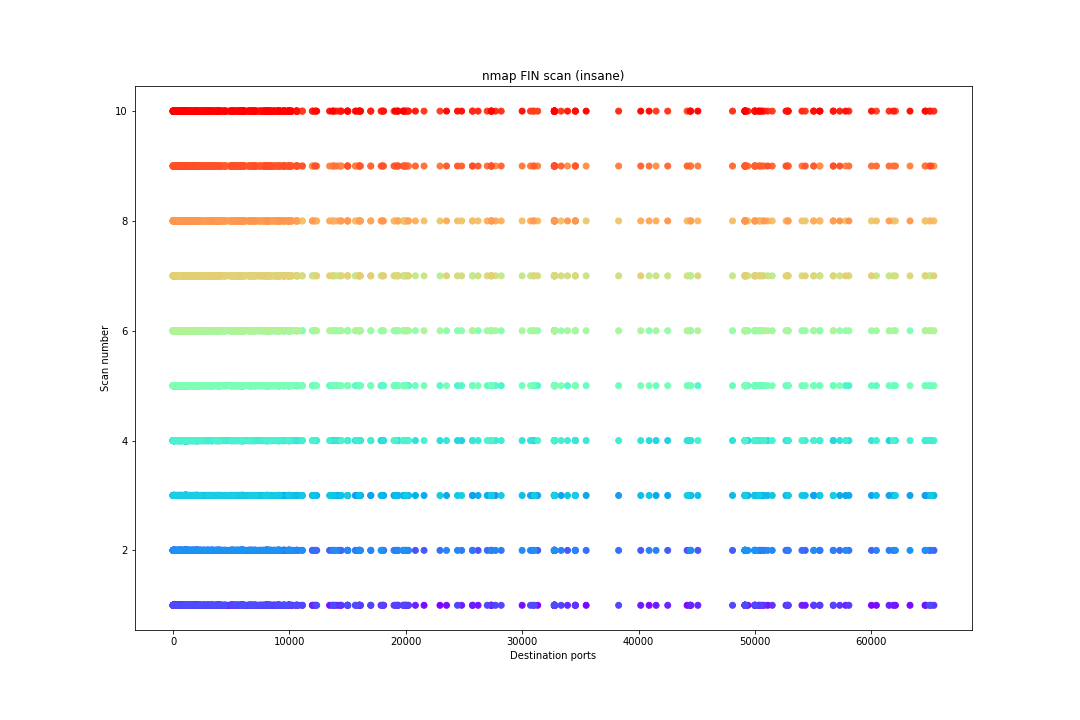
\includegraphics[width=8.2cm]{images/analysis/finscan/insane/ScanNrDstPort.png} }
    \subfloat[ping scan aggressive\label{fig:PngAgrScnDst}]{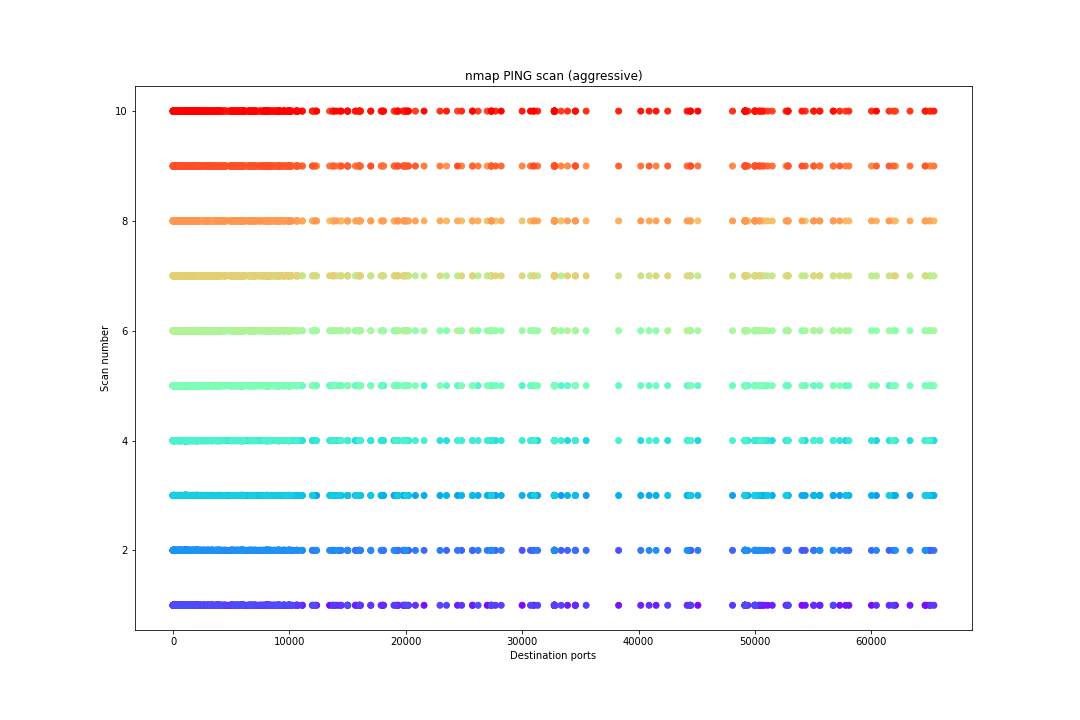
\includegraphics[width=8.2cm]{images/analysis/pingscan/aggressive/ScanNrDstPort.png} }\\
    \subfloat[service discovery normal\label{fig:SvcNorScnDst}]{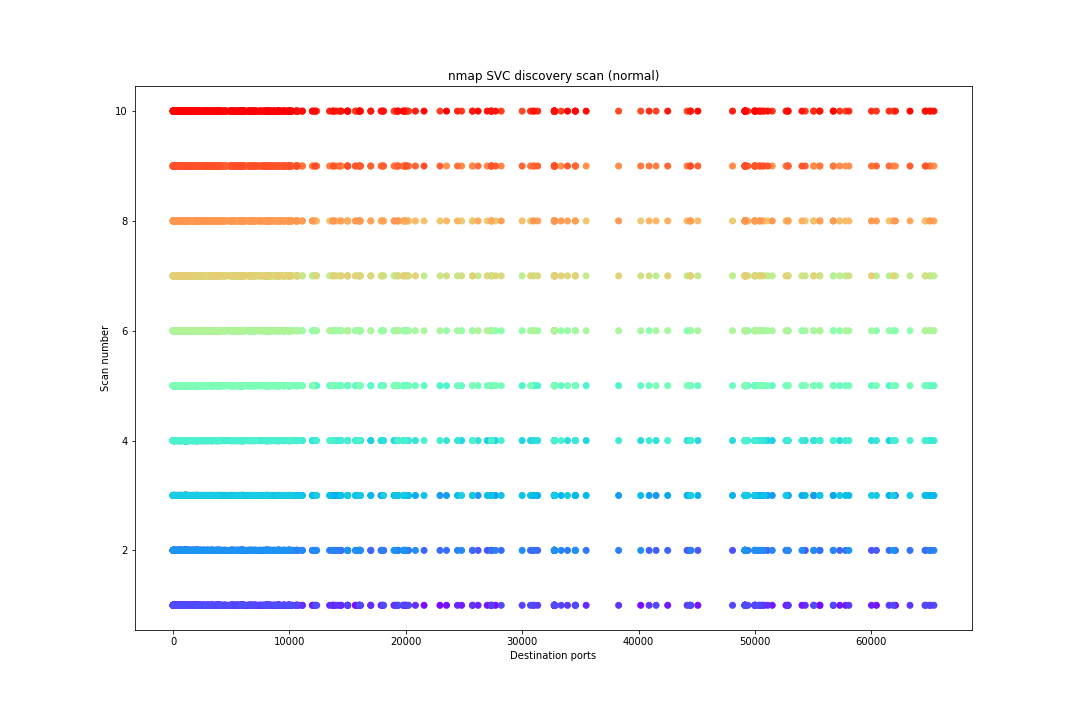
\includegraphics[width=8.2cm]{images/analysis/svcscan/normal/ScanNrDstPort.png} }
    \subfloat[null scan polite\label{fig:NullPolScnDst}]{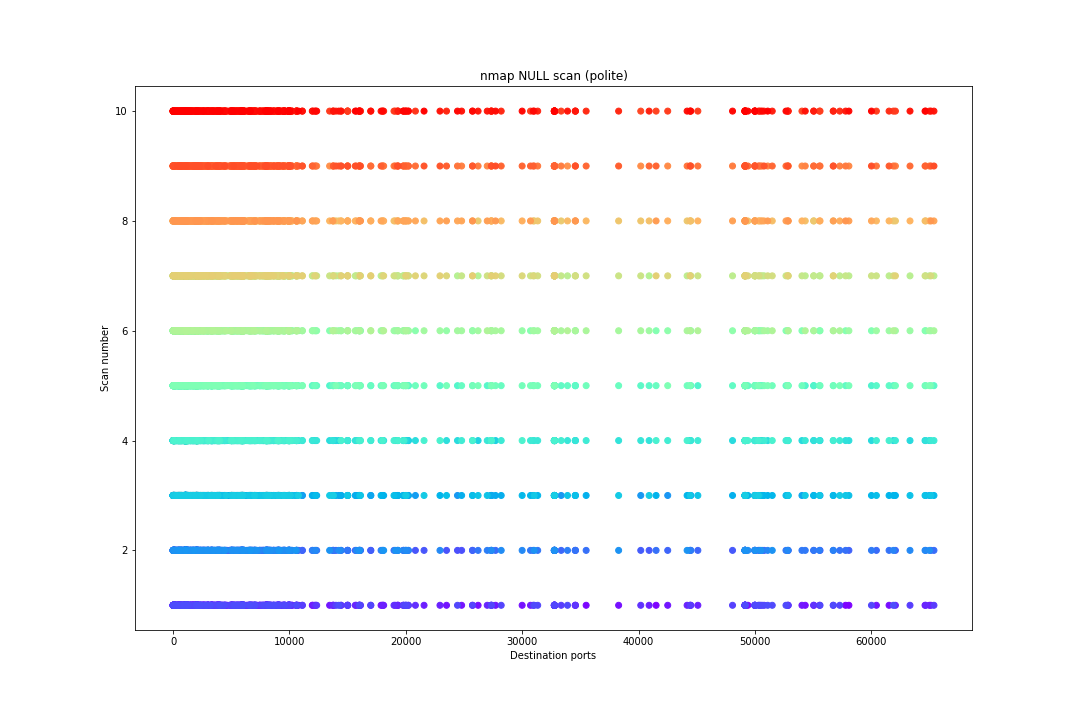
\includegraphics[width=8.2cm]{images/analysis/nullscan/polite/ScanNrDstPort.png} }\\
    \subfloat[xmas scan sneaky\label{fig:XmasSneScnDst}]{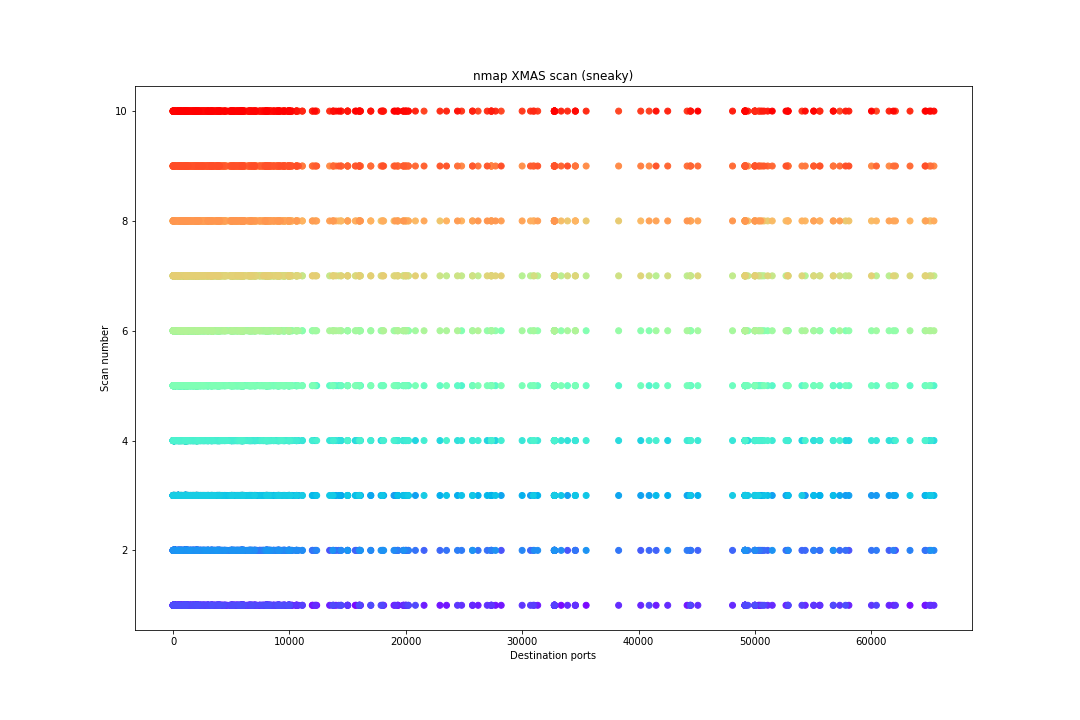
\includegraphics[width=8.2cm]{images/analysis/xmasscan/sneaky/ScanNrDstPort.png} }
    \subfloat[TCP SYN paranoid\label{fig:TcpParScnDst}]{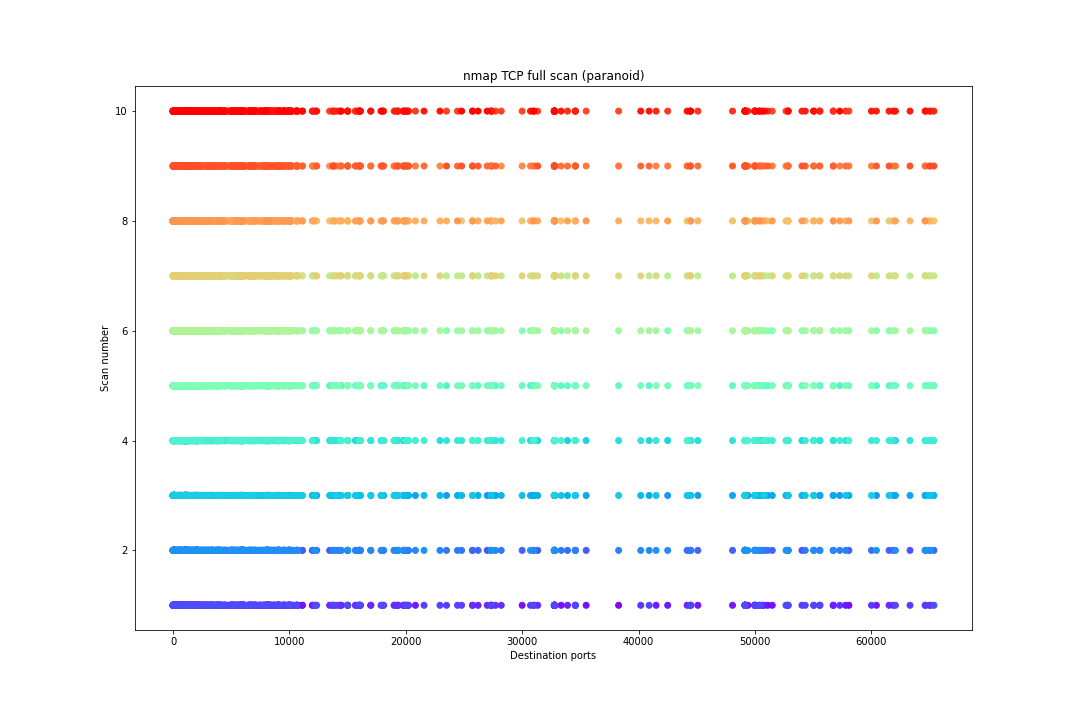
\includegraphics[width=8.2cm]{images/analysis/tcpsynscan/paranoid/ScanNrDstPort.png} }
    \caption{Scan number and destination port diagram}%
    \label{fig:ScanNumberDstPort}%
\end{figure}

The figure does not clearly point out the sequence of which ports are targeted in sequence. This is elaborated in section \ref{s:PortSequences}. It neither tells anything about how many destination ports is targeted. A code snippet could be implemented to go through which ports are not targeted, as seen in listing \ref{lst:UnusedPorts}.

\begin{listing}[!ht]
\caption{Print values and counts of unused ports}
\label{lst:UnusedPorts}
\begin{minted}{python}
unused_ports = []
used_ports = []
for x in range(1, 65536):
    if x not in tcp_dports:
        unused_ports.append(x)
    elif x in tcp_dports:
        used_ports.append(x)

print(len(unused_ports)) # print the count of unused ports
print(unused_ports) # print all the unused ports
print(len(used_ports)) # print the count of used ports
print(used_ports) # print all used ports
\end{minted}
\end{listing}

The code in listing \ref{lst:UnusedPorts} were implemented into the Jupyter notebooks for the scans seen in figure \ref{fig:ScanNumberDstPort}. Each of these notebooks reported an unused port count of 64535 ports for each scan where the scanning type used and the timing template used were irrelevant, and the count stayed the same.

\vfill
\clearpage

\newpage
\vfill